\documentclass[11pt]{article}
\usepackage[         %
	a4paper,         %
	centering,       %
	textwidth=14cm,  %
	top=4.6cm,       %
	headsep=.6cm,    %
	footnotesep=1cm, %
	footskip=0.6cm,  %
	bottom=3.8cm     %
]{geometry}
\usepackage[slovak]{babel}
\usepackage[T1]{fontenc}
\usepackage[utf8]{inputenc}
\usepackage{graphicx}
\usepackage{booktabs}
\usepackage{caption}
\usepackage{longtable}

\title{JChat \\ \large{Dokumentácia}}
\author{Ondřej Kipila}

\begin{document}
\maketitle

\pagebreak

\section{Zadanie projektu}
Program bude určený na zabezpečenie komunikácie viacerých používateľov v~reálnom čase.
Prostredníctvom programu bude možné posielať niekoľko typov správ (textové,
obrázkové\dots), pričom budú používateľom zobrazované rôznym spôsobom podľa typu
správy.

Používatelia budú mať možnosť vytvárať a pripájať sa do \uv{miestností}, pričom
správy posielané v~určitej miestnosti budú dostupné len pre používateľov, ktorí
sú k~danej miestnosti pripojení. Program bude umožňovať aj posielanie správ
určených len pre konkrétneho používateľa (pre ostatných nebude viditeľná).

Používatelia tiež budú mať rozdielne oprávnenia, napr.\ na zablokovanie určitého
užívateľa, atď.

Program bude pracovať v~textovom aj grafickom režime.

\pagebreak

\section{Návod na použitie programu}

Po spustení programu sa zobrazí prihlasovacie okno (obr.~\ref{fig:loginwindow}).
Pri výbere voľby \uv{Start server} bude aplikácia spustená v~režime server-klient,
v~opačnom prípade bude spustená v~režime klient. Po stlačení tlačidla
\uv{Connect} prebehne prihlásenie a zobrazí sa hlavné okno aplikácie
(obr.~\ref{fig:mainwindow}).

\bigskip

\begin{centering}
	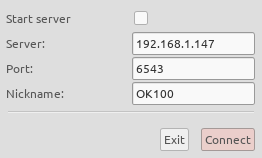
\includegraphics[scale=0.75]{login.png}
	\captionof{figure}{Prihlasovacie okno}
	\label{fig:loginwindow}

	\bigskip

	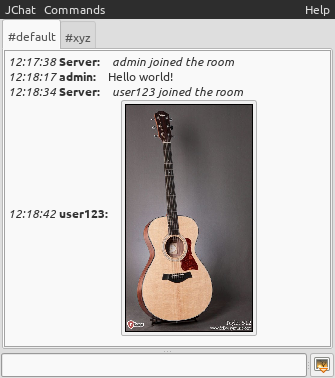
\includegraphics[scale=0.75]{main.png}
	\captionof{figure}{Hlavné okno aplikácie}
	\label{fig:mainwindow}
\end{centering}

\bigskip

Hlavné okno je rozdelené na niekoľko častí. V~hornej časti okna je hlavná ponuka
a záložky miestností. V~strednej časti sa zobrazujú správy vo vybranej
miestnosti. V~dolnej časti okna sa nachádza textové pole na odosielanie
textových správ. Tlačidlo \uv{Send image\dots} v~pravom dolnom rohu je určené
na odosielanie grafických správ.

V~textovom poli je tiež možné používať rôzne príkazy (tab.~\ref{tab:prikazy}),
ktoré sú tiež dostupné z~ponuky \uv{Commands}.

\begin{longtable}{p{1cm} p{5cm} p{7cm}}
	\toprule
	Príkaz & Syntax príkazu & Popis príkazu \\
	\midrule
	\texttt{block} & \texttt{/block MENO-POUZIVATELA ZABLOKOVAT-ODBLOKOVAT} &
	Zablokovanie/odblokovanie používateľa v~danej miestnosti. Parameter
	\texttt{MENO-POUZIVATELA} udava meno používateľa, parameter
	\texttt{ZABLOKOVAT-ODBLOKOVAT}
	udáva, či bude používateľ zablokovaný alebo odblokovaný (\texttt{true} pre
	zablokovanie, \texttt{false} pre odblokovanie). Príkaz je dostupný len pre
	správcu miestnosti (používateľ, ktorý ju vytvoril).\\

	\texttt{join} & \texttt{/join NAZOV-MIESTNOSTI} & Pripojenie používateľa
	k~miestnosti. Parameter \texttt{NAZOV-MIESTNOSTI} udáva názov miestnosti ku
	ktorej bude používateľ pripojený. V~prípade, že miestnosť ešte nebola
	vytvorená, používateľ sa automaticky stane jej správcom. \\

	\texttt{leave} & \texttt{/leave} & Odpojenie používateľa od miestnosti.
	Používateľ sa odpojí od miestnosti v~ktorej odoslal tento príkaz. \\

	\texttt{rooms} & \texttt{/rooms} & Vypíše zoznam všetkých miestností. \\

	\texttt{stats} & \texttt{/stats} & Vypíše informácie o~serveri. \\

	\texttt{users} & \texttt{/users} & Vypíše zoznam používateľov ktorí sú
	pripojení k~miestnosti, v~ktorej bol príkaz odoslaný. \\
	\bottomrule
	\caption{Prehľad príkazov}
	\label{tab:prikazy}
\end{longtable}

\pagebreak

\section{Štruktúra systému}

\subsection{Sieťová časť}

\begin{figure}[h]
	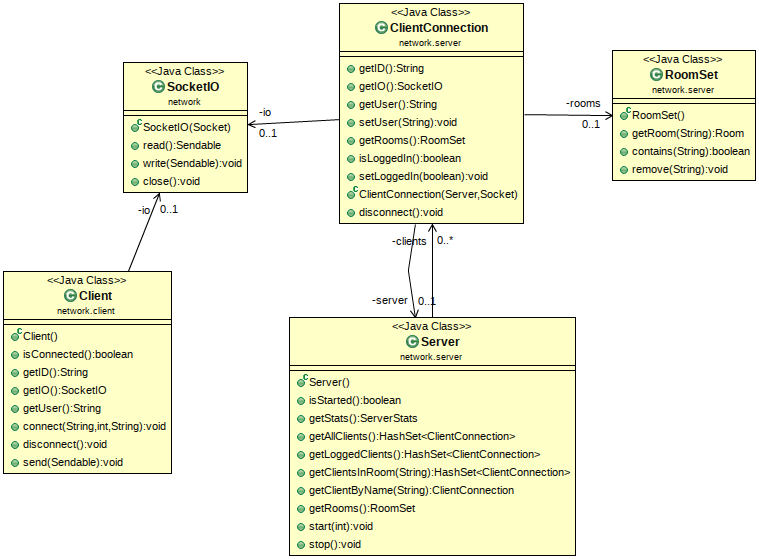
\includegraphics[width=\textwidth]{UML-network.png}
	\caption{Diagram najdôležitejších tried}
\end{figure}

\begin{itemize}
	\item \texttt{Server} --- Hlavná trieda servera. Server je schopný spracovať max. 10
	      súčasných požiadaviek na pripojenie. Server si uchováva referenciu na
		  objekt typu \texttt{ClientConnection} pre každého pripojeného klienta.
	\item \texttt{Client} --- Hlavná trieda klienta. Príjem a odosielanie správ je
	      realizovaný prostredníctvom zapúzdreného objektu typu
		  \texttt{SocketIO}. Príjem správ zo servera prebieha v~samostatnom vlákne.
	\item \texttt{SocketIO} --- Zabezpečuje príjem a odosielanie
	      serializovateľných objektov prostredníctvom socketu.
	\item \texttt{ClientConnection} --- Prepojenie servera a klienta. Príjem správ od
	      klienta prebieha v~samostatnom vlákne.
	\item \texttt{RoomSet} --- Obsahuje zoznam miestností ku ktorým je daný
	      používateľ pripojený.
\end{itemize}

\subsubsection{Správy}
\begin{figure}[h]
	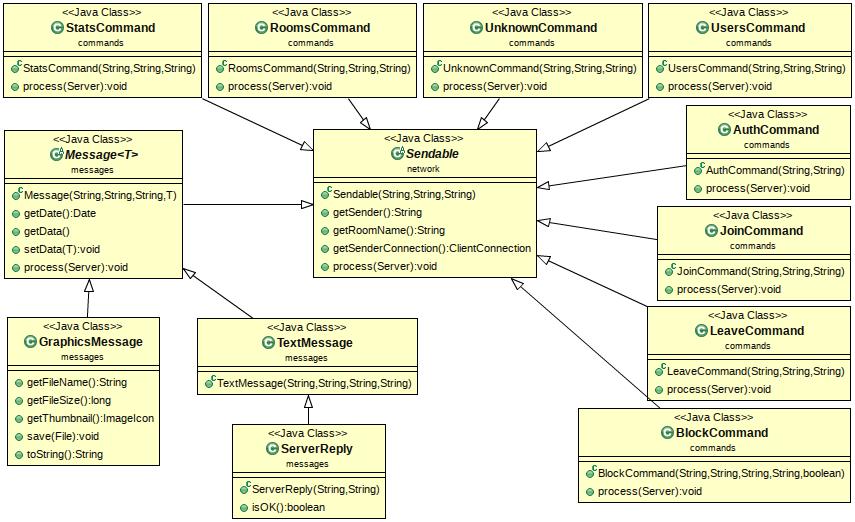
\includegraphics[width=\textwidth]{UML-msg.png}
	\caption{Diagram najdôležitejších tried}
\end{figure}

\begin{itemize}
	\item \texttt{Sendable} --- Abstraktná trieda objektu ktorý je možné
	      posielať.
	\item \texttt{Message} --- Abstraktná trieda správy generického typu.
	\item \texttt{GraphicsMessage} --- Grafická správa.
	\item \texttt{TextMessage} --- Textová správa.
	\item \texttt{ServerReply} --- Textová správa posielaná serverom.
	\item \texttt{AuthCommand} --- Príkaz pre prihlásenie.
	\item \texttt{BlockCommand} --- Príkaz pre zablokovanie/odblokovanie
	      používateľa.
	\item \texttt{JoinCommand} --- Príkaz pre pripojenie k~miestnosti.
	\item \texttt{LeaveCommand} --- Príkaz pre odpojenie od miestnosti.
	\item \texttt{RoomsCommand} --- Príkaz pre výpis miestností.
	\item \texttt{StatsCommand} --- Príkaz pre výpis informácií o~serveri.
	\item \texttt{SyntaxErrorCommand} --- Príkaz s~chýbajúcimi parametrami je
	      nahradený týmto príkazom.
	\item \texttt{UnknownCommand} --- Neznámy príkaz je nahradený týmto
	      príkazom.
	\item \texttt{UsersCommand} --- Príkaz pre výpis používateľov.
\end{itemize}

\subsection{Aplikačná časť}

\begin{figure}[h]
	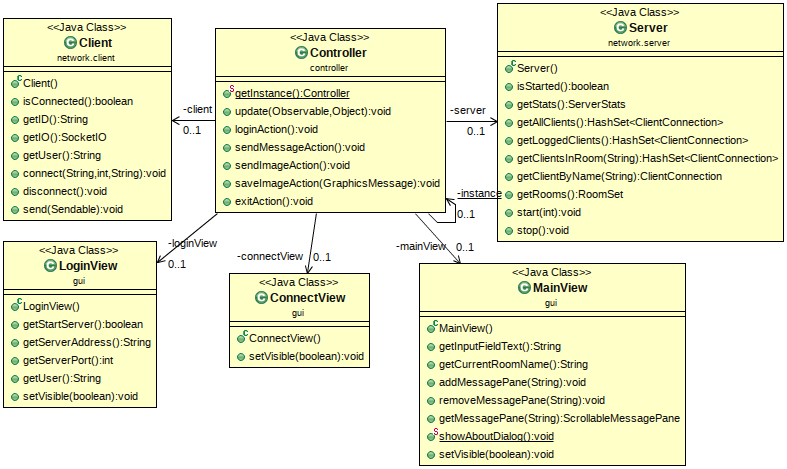
\includegraphics[width=\textwidth]{UML-app.png}
	\caption{Diagram najdôležitejších tried}
\end{figure}

\begin{itemize}
	\item \texttt{Controller} --- Zabezpečuje prepojenie grafického používateľského
	      rozhrania a modelu (klient, server).
	\item \texttt{Client} --- Hlavná trieda klienta.
	\item \texttt{Server} --- Hlavná trieda servera.
	\item \texttt{LoginView} --- Prihlasovacie okno.
	\item \texttt{ConnectView} --- Okno zobrazené v~priebehu prihlasovania.
	\item \texttt{MainView} --- Hlavné okno aplikácie.
\end{itemize}

\pagebreak

\section{Kritériá hodnotenia}

\paragraph{Hlavné kritériá}
Aplikácia podľa môjho názoru splňuje všetky hlavné kritériá hodnotenia.
\begin{itemize}
	\item Aplikácia zodpovedá spresnenému zadaniu, jediná chýbajúca vlastnosť je
	      textové používateľské rozranie, ktoré nakoniec nebolo realizované kvôli
	      nemožnosti zobraziť grafické správy
	\item Sú použité objektovo-orientované mechanizmy Javy (dedenie,
	      polymorfizmus, zapuzdrenie, agregácia)
	\item Zdrojový kód obsahuje bežné aj Javadoc komentáre
\end{itemize}

\paragraph{Dodatočné kritériá}
\begin{itemize}
	\item Použité návrhové vzory --- MVC, factory, observer, proxy, singleton
	\item Kód je organizovaný do balíkov
	\item Sú ošetrené mimoriadne stavy, vrátane vlastných výnimok
	\item Grafické používateľské rozhranie je oddelené od aplikačnej logiky
	      pomocou návrhového vzoru MVC
	\item Využitie viacniťovosťi, dynamické vytváranie vlákien za behu aplikácie
	\item Použitie pokročilých mechanizmov Javy --- RTTI, vhniezdené triedy,
	      generickosť vo vlastných triedach
\end{itemize}

\end{document}
